\subsection{Colors > Height Ramp}
\label{subsection:heightRamp}

\begin{figure}[!htb]
\begin{center}
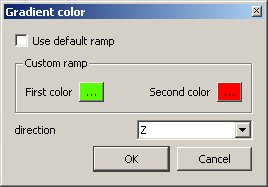
\includegraphics[width=0.4\textwidth]{Partie3_Fonctions/heightRampDlg.png}
\caption{\label{fig:heightRampDlg}Interface de s�lection d'une rampe de couleur}
\end{center}
\end{figure}

\begin{figure}[!htb]
\begin{center}
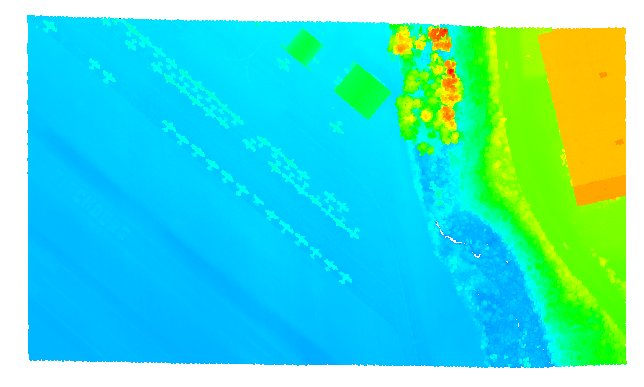
\includegraphics[width=0.5\textwidth]{Partie3_Fonctions/HeightRamp.jpg}
\caption{\label{fig:heightRampExample}Exemple d'un d�grad� selon Z (couleurs par d�faut)}
\end{center}
\end{figure}

\index{couleurs}
L'utilisateur � le choix entre appliquer une rampe par d�faut (figure~\ref{fig:heightRampExample})
ou alors une rampe dont il d�finit les deux couleurs extr�mes (figure~\ref{fig:heightRampDlg}).
Il faut pour cela d�sactiver la case � cocher \emph{Use default ramp}. Les deux couleurs extr�mes du d�grad� peuvent alors �tre d�finies en cliquant sur les boutons color�s \emph{First color} et \emph{Second color} (qui
font appara�tre des interfaces de s�lection de couleur �quivalentes � celle de la m�thode \emph{Set Unique} - Cf. section~\ref{subsection:setUniqueColor}).\\
\par
Via la liste d�roulante \textit{direction}, l'utilisateur doit aussi d�finir selon quelle direction le d�grad� sera appliqu� (parmi les 3 directions principales : X, Y ou Z).
